\documentclass[11pt]{article}

\usepackage[letterpaper, margin=1in]{geometry}

\usepackage[spanish]{babel}
\usepackage[utf8]{inputenc}
\usepackage{multirow}
\usepackage{tabularx}
\usepackage{longtable}



%Figuras
\usepackage{graphicx, subfigure}
\usepackage[]{tikz}
\usepackage{pbox}

%Matemática
\usepackage{amsmath}
\usepackage{amssymb}

%Símbolos mate extra (alfabetos, etc.)
\usepackage{mathrsfs}


%Algoritmos
\usepackage{float}
\usepackage{algorithm}
\usepackage{algorithmicx}
\usepackage{algpseudocode}
\usepackage{listings}


\usepackage{color}
\usepackage{hyperref}

\usepackage{mdframed}
\usepackage{tcolorbox}
\usepackage{multicol}
\usepackage{booktabs}
\usepackage{tabulary}
\definecolor{darkblue}{rgb}{0 , 0.054 , 0.196}



\title{Reporte de Laboratorio 0\\Manejo de versiones, compilación y documentación}
\author{Dunia Barahona - B40806}
%otro autor se pondría así \author{nombre1\\nombre2}
\begin{document}

\maketitle
\hrule
\hrule
\tableofcontents
\hspace{5mm}
\hrule
\hrule

\section{Código}
\begin{enumerate}
	\item Se subieron a repositorios tres programas y su documentación:
	
	\begin{figure}[H]
		\centering
		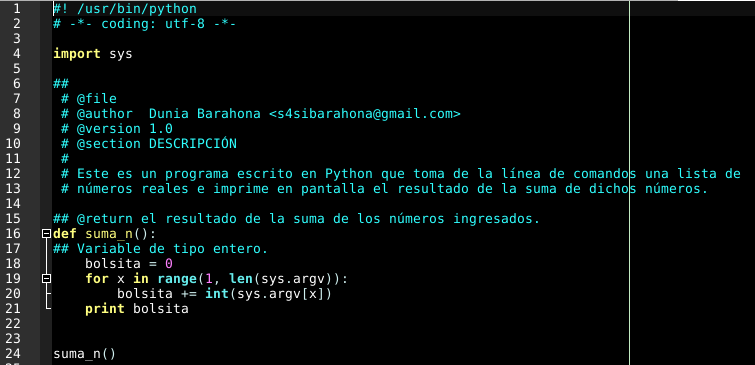
\includegraphics[scale=0.6]{cdPy.png}
		\caption{suma.py}
		\label{fig:cPy}
	\end{figure}
	
	\begin{figure}[H]
		\centering
		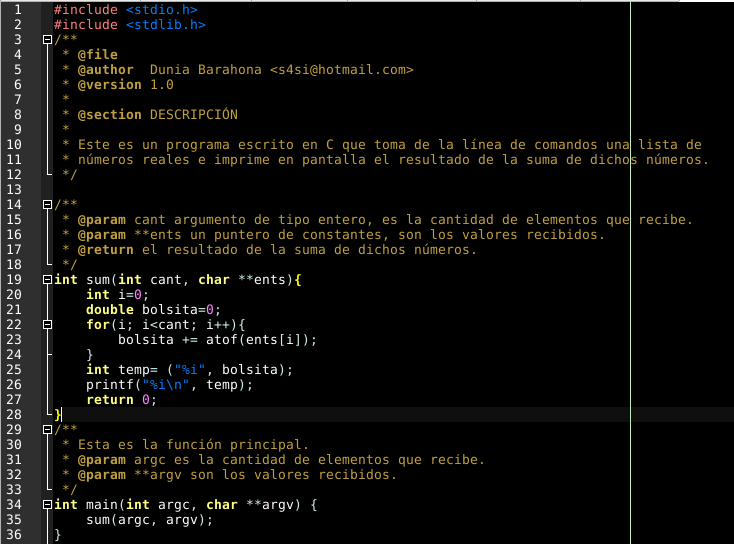
\includegraphics[scale=0.6]{cdC.png}
		\caption{suma.c}
		\label{fig:cPy}
	\end{figure}
	
	\begin{figure}[H]
		\centering
		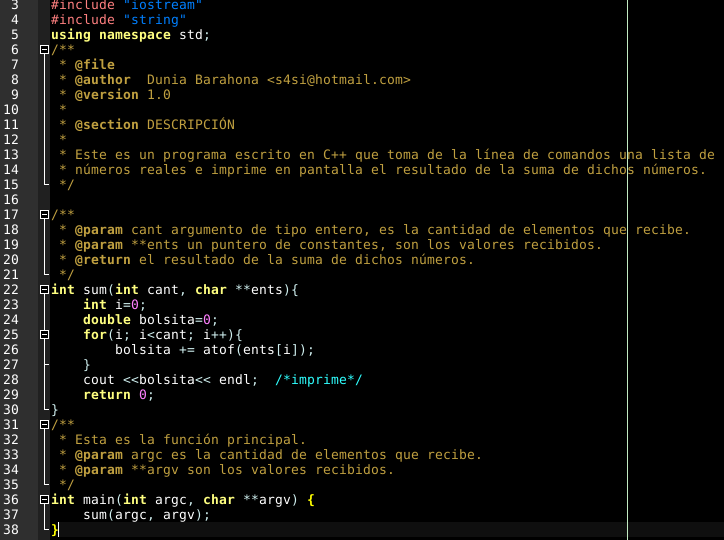
\includegraphics[scale=0.6]{cdCpp.png}
		\caption{suma.cpp}
		\label{fig:cPy}
	\end{figure}
	
	\item Se creó un \textbf{Makefile} con cuatro \textit{targets}:
	\begin{itemize}
		\item Compilar.
		\item Borrar.
		\item Ejecutar.
		\item All: este se encarga de correr los primeros tres en orden.
	\end{itemize}
\end{enumerate}

\section{GitHub}
Documentación del tutorial:

\begin{figure}[H]
	\centering
	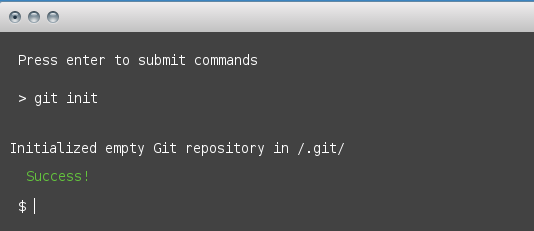
\includegraphics[scale=0.8]{git_1.png}
	\caption{Inicialización de repositorio}
	\label{fig:c1}
\end{figure}

\begin{figure}[H]
	\centering
	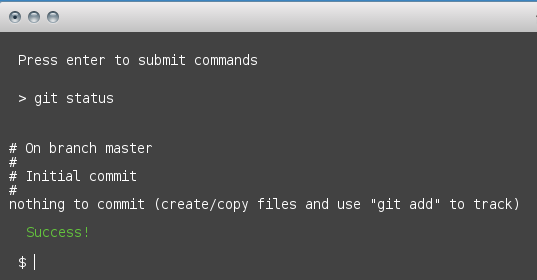
\includegraphics[scale=0.8]{git_2.png}
	\caption{git status}
	\label{fig:c2}
\end{figure}

\begin{figure}[H]
	\centering
	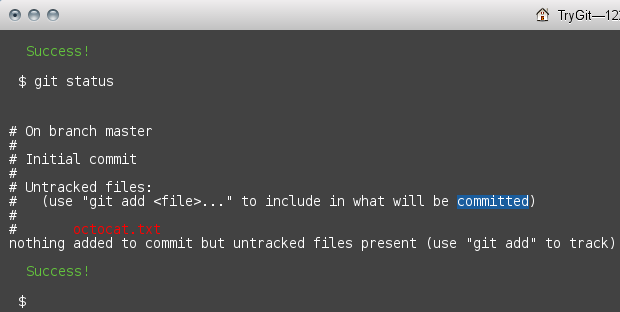
\includegraphics[scale=0.8]{git_3.png}
	\caption{git status}
	\label{fig:c3}
\end{figure}

\begin{figure}[H]
	\centering
	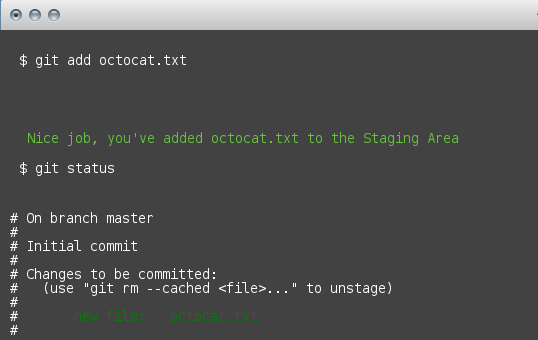
\includegraphics[scale=0.8]{git_4.png}
	\caption{Hacer que revise cambios en archivo}
	\label{fig:c4}
\end{figure}

\begin{figure}[H]
	\centering
	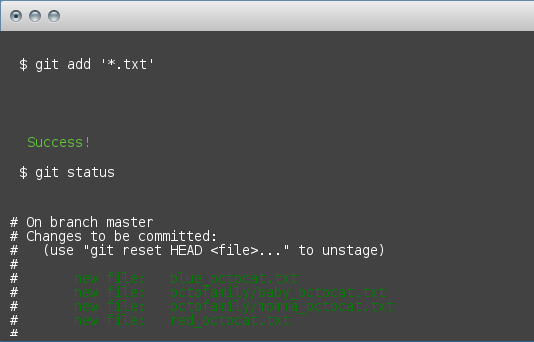
\includegraphics[scale=0.8]{git_5.png}
	\caption{Hacer que revise cambios en todos los archivos .txt}
	\label{fig:c5}
\end{figure}

\begin{figure}[H]
	\centering
	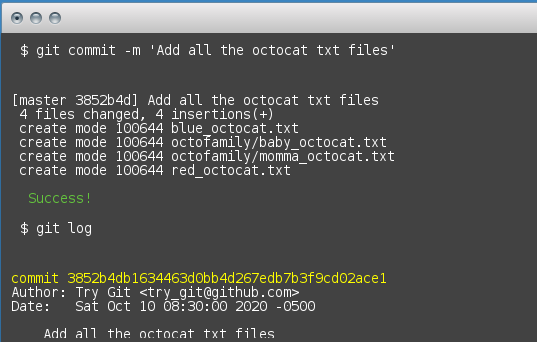
\includegraphics[scale=0.8]{git_6.png}
	\caption{git commit}
	\label{fig:c6}
\end{figure}

\begin{figure}[H]
	\centering
	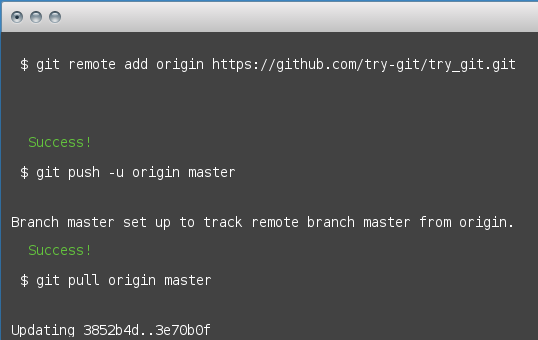
\includegraphics[scale=0.8]{git_7.png}
	\caption{Repositorio remoto}
	\label{fig:c7}
\end{figure}

\begin{figure}[H]
	\centering
	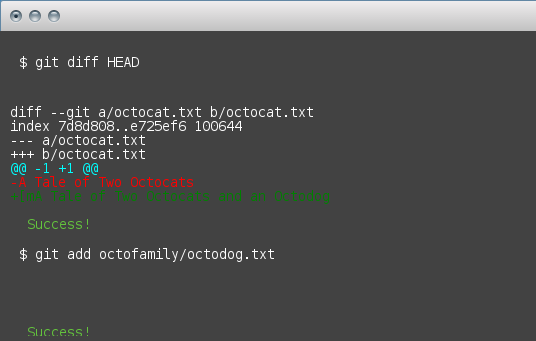
\includegraphics[scale=0.8]{git_8.png}
	\caption{Diferencias desde el último commit}
	\label{fig:c8}
\end{figure}

\begin{figure}[H]
	\centering
	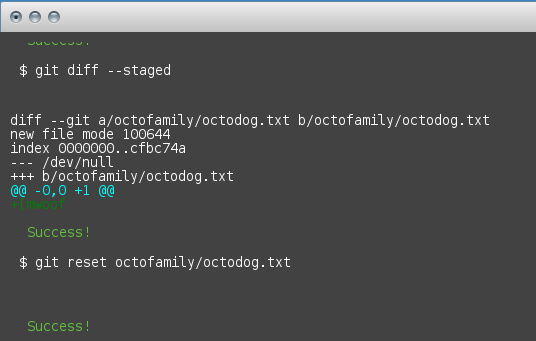
\includegraphics[scale=0.8]{git_9.png}
	\caption{Cambios que se han dado}
	\label{fig:c9}
\end{figure}

\begin{figure}[H]
	\centering
	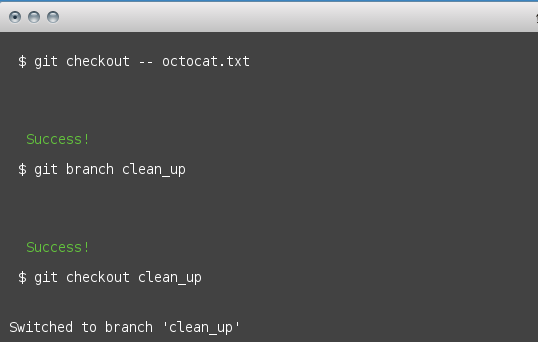
\includegraphics[scale=0.8]{git_10.png}
	\caption{git checkout}
	\label{fig:c10}
\end{figure}

\begin{figure}[H]
	\centering
	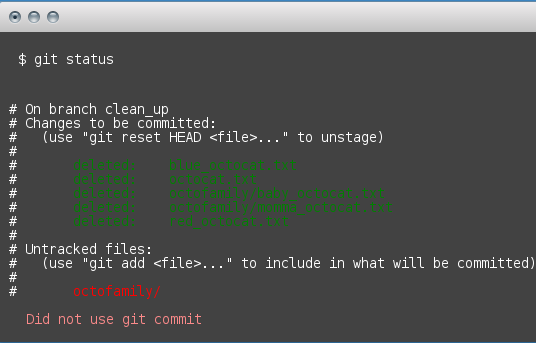
\includegraphics[scale=0.8]{git_11.png}
	\caption{git status}
	\label{fig:c11}
\end{figure}

\begin{figure}[H]
	\centering
	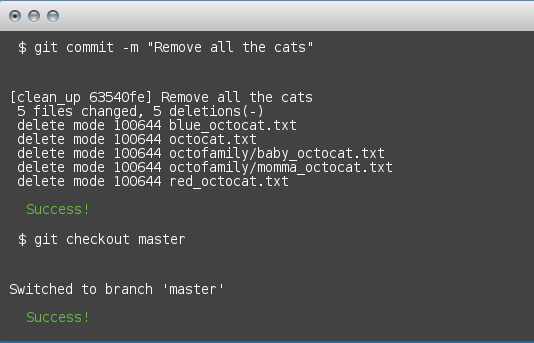
\includegraphics[scale=0.8]{git_12.png}
	\caption{git commit}
	\label{fig:c12}
\end{figure}

\begin{figure}[H]
	\centering
	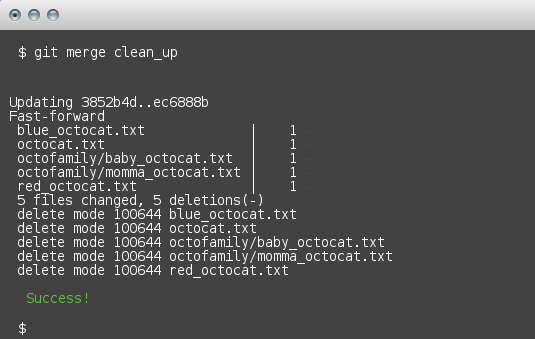
\includegraphics[scale=0.8]{git_13.png}
	\caption{Unión de \textit{branches}}
	\label{fig:c13}
\end{figure}

\begin{figure}[H]
	\centering
	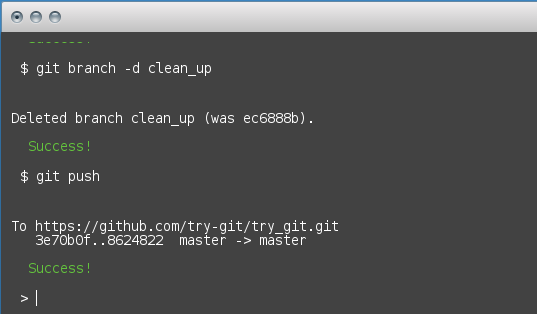
\includegraphics[scale=0.8]{git_14.png}
	\caption{Eliminar rama}
	\label{fig:c14}
\end{figure}

\section{Conclusiones}
\begin{enumerate}
	\item Doxygen es una herramienta muy completa, que facilita el proceso de documentación.
	\item \LaTeX{} es un programa que permite crear documentos de buena calidad de manera sencilla.
	\item GitHub requiere de práctica para hacer uso de todas las opciones que ofrece.
\end{enumerate}
\end{document}
